\documentclass[a4paper, 11pt, normalem]{report}

\usepackage{../../../LaTeX-Templates/Notes}
\usepackage{subfiles}
\usepackage{epigraph}

\setlength{\epigraphwidth}{\textwidth}
\titleformat{\part}[display]
{\normalfont\huge\filcenter\bfseries\thispagestyle{epigraph}}
{\partname\ \thepart}
{20pt}
{\Huge}
\titlespacing*{\part}{0pt}{0pt}{40pt}

\title{Atoms, Lasers, and Qubits \vspace{-20pt}}
\author{Dr Weatheril and Prof Adams}
\date{\vspace{-15pt}Michaelmas Term 2019 - Epiphany Term 2020}
\rhead{\hyperlink{page.1}{Contents}}

\begin{document}

\maketitle
%\tableofcontents

\epigraphhead[200]{\hfil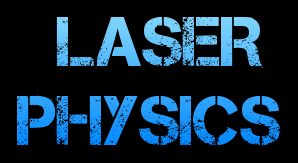
\includegraphics{lasers.png}\hfil}
\part{}
\chapter{}
\begin{itemize}
    \item \textbf{Note:} The course will be more reading based than math based. 
Read the references on each summary sheet. 
    \item Need light oscillation, not just amplification.  
    \item 1 in $10^{18}$ atomic clock accuracy.
    \item LD: laser diode
    \item Non-linear crystals allow different wavelengths
    \item Laser transitions based on E group of materials
    \item Learn the unit conversions
    \item Magneto-optical trap to cool atoms
    \item Optical frequency comb $\to$ accurate measurement of wavelength of light 
    \item Sodium atoms in upper atmosphere which we fluoresce for AO
    \item \textbf{LEARN!} Q on paper always - contents of a laser
        \begin{enumerate}
            \item More in excited state than ground
            \item Pump gets energy in
            \item Mirrors to make light bounce back and forward
        \end{enumerate}
\end{itemize}

\section{Introduction to lasers}
Lasers - coherence $\to$ 2 types - longitudinal and transverse
\begin{itemize}
    \item Lasers are highly coherent, both transversely and longitudinally. 
        Longitudinal and temporal coherence is related to linewidth, and will be discussed. 
        Coherence length $l_c$ and coherence time $\tau_c$ are the distance and time over which a coherent wave maintains a specified degree of coherence, i.e. when its phase is predictable. 
\end{itemize}
\begin{multicols}{2}
\begin{figure}[H]
    \centering
    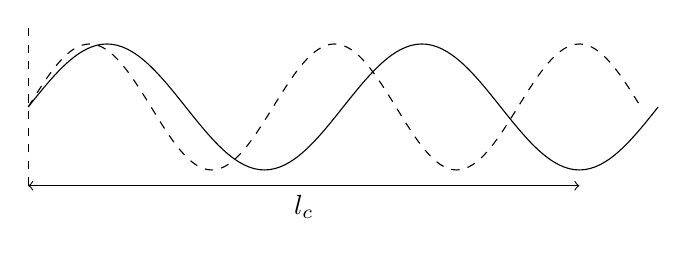
\begin{tikzpicture}
        \draw[dashed] (0,0) -- (0,2);
        \draw[<->] (0,0) -- (7,0) node[anchor=north,midway] {$l_c$};
        \draw (0,1) sin (1,1.8) cos (2,1) sin (3,0.2) cos (4,1) sin (5,1.8) cos (6,1) sin (7,0.2) cos (8,1);
        \draw[dashed] (0,1) sin (0.78,1.8) cos (1.56,1) sin (2.33,0.2) cos (3.11,1) sin (3.89,1.8) cos (4.67,1) sin (5.44,0.2) cos (6.22,1) sin (7,1.8) cos (7.78,1);
    \end{tikzpicture}
\end{figure}
\columnbreak
Coherence length and time:
\begin{align}
    l_c &= \frac{2\pi c}{\delta\om},~~  \tau_c = \frac{2\pi}{\delta\om}
\end{align}
\end{multicols}
\begin{itemize}
    \item Can't have an infinitely narrow spectrum. 
        Monochromaticity - laser has a spectral linewidth $\delta\om$, this is much smaller than the actual carrier/centre frequency. $\delta\om\ll\om_0$ for a laser where $\om_0$ is the centre frequency. 
        From mHz to GHz in range. 
    \item Highly directional beam $\to$ energy contained in one region. 
\end{itemize}
Directionality:
\begin{itemize}
    \item Lasers have highly directional beams that diverge due to diffraction
    \item Beam will be larger
    \item Waist of beam, $2\om_0$.
\end{itemize}
\begin{figure}[H]
    \centering
    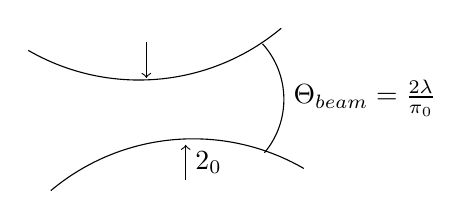
\begin{tikzpicture}
        \draw (0,1) arc (240:310:80pt);
        \draw (3.5,-0.5) arc (60:130:80pt);
        \draw (3,-0.3) arc (-40:42:30pt) node[anchor=west,midway] {$\Theta_{beam} = \frac{2\lambda}{\pi\om_0}$};
        \draw[->] (1.5,1.1) -- (1.5,0.65);
        \draw[->] (2,-0.65) -- (2,-0.2) node[anchor=west,midway] {$2\om_0$};
    \end{tikzpicture}
\end{figure}
\begin{itemize}
    \item All in a very low frequency range $\to$ all energy oscillating in small aarea in small frequency range - useful applications. 
\end{itemize}
Brightness:
\begin{itemize}
    \item Lasers are spectrally bright
    \item Definition of brightness - amount of power in particular area (solid angle) of the beam:
        \begin{equation}
            B_\om = \frac{P}{A\Delta\Om\Delta\om},
        \end{equation}
        where $A$ is the area, $\Delta\Om$ is the solid angle, and $\Delta\om$ is the linewidth. 
\end{itemize}
Electromagnetic Field Modes - not examinable:
\begin{itemize}
    \item 1st Chapter of 'Laser Physics' book
    \item Planck's radiation law
    \item Each unique solution of field is EM mode
    \item $L^3$ factored out when divided by volume
    \item Modes exist with or without energy
\end{itemize}


\chapter{Einstein's rate equations}
A laser requirs amplification due to stimulated emission of radiation. 
\textit{Doodle of two energy levels with E,g,N 1 and 2.}
\begin{align}
    E_2 - E_1 = \hbar\om_{12}
\end{align}
\begin{enumerate}
    \item Spontaneous emission: Atom in some excited state, until some time later where it spontaneously decays into a lower state, with a photon emitted with energy shown in Eq (2.1). 
        Rates: $A_{21}$ per $N_i$ atoms, or $A_{21}N_2$ per $m^3$.
    \item Absorption: Excite into excited state using energy of photon. 
        Rates: $B_{12}\rho(\om_{12})$, $B_{12}\rho(\om_{12})N_2$.
    \item Stimulated emission: At the initial time we have an atom in an excited state which we then apply a radiated field (photon) to. Later, the atom will decay into a lower state and there will be two outgoing photons - they have been emitted into the same mode.
        Rates: $B_{21}\rho(\om_{12})$, $B_{21}\rho(\om_{12})N_2$. Note: 
        \begin{itemize}
            \item Here, $\rho(\om_{12})$ is the spectral energy density - the energy density, per unit angular frequency range at $\om$, with units of $J\,m^{-3}\,s$.
            \item Generally, the light being used here is broad-band.
        \end{itemize}
\end{enumerate}

\section{Apply the 3 processess}
\textit{Doodle going through $A_{21}$ to $B_{12}$ to $B_{21}$.}
Conservation of atom number:
\begin{align}
    \frac{dN_2}{dt} &= -\frac{dN_1}{dt} \\
    N_1 + N_2 &= N = \text{const} \\
    N_1B_{12}\rho(\om_{12}) &= N_2A_{21} + N_2B_{21}\rho(\om_{12})
\end{align}
Rearrange for the spectral energy density:
\begin{align}
    \rho(\om_{12}) &= \frac{N_2A_{21}}{N_1B_{12}-N_2B_{21}} = \frac{\frac{A_{21}}{B_{21}}}{\frac{N_1}{N_2}\frac{B_{12}}{B_{21}} - 1}
\end{align}
Substitute using Boltzmann Law:
\begin{align}
    \frac{N_2}{N_1} &= \frac{g_2}{g_1}\exp\left(-\frac{\hbar\om_{12}}{k_BT}\right) \\
    \implies \rho(\om_{12}) &= \frac{\frac{A_{21}}{B_{21}}}{\frac{g_1}{g_2}\frac{B_{12}}{B_{21}}\exp\left(\frac{\hbar\om_{12}}{k_BT}\right) - 1}
\end{align}
Now look at Planck's Law:
\begin{align}
    \rho(\om) &= \frac{\hbar\om^3}{\pi^2c^3} \frac{1}{\exp\left(\frac{\hbar\om}{k_BT}\right) - 1}
\end{align}
Einstein realised there must be an extra condition to switch between these two forms.
This reveals:
\begin{align}
    g_1B_{12} &= g_2B_{21} \\
    A_{21} &= \frac{\hbar\om_{12}^3}{\pi^2c^3}B_{21}
\end{align}
Notes:
\begin{itemize}
    \item Effectively only 1 coefficient as if we know A, we know B. 
    \item $A_{21}$ is the radiative decay rate,
        \begin{equation}
            A_{21} = \frac{1}{\tau_2}
        \end{equation}
    \item B has units $m^3\,J^{-1}\,s^{-2}$.
    \item A and B are constants for a particular atom.
    \item From the $\om^3$ term, we can see that an infrared transition may decay very fast, but a microwave transition may decay very slow. 
    \item Ratio of $A/B \propto \om^3$ - lasers at high requency harder to achieve.
    \item The principle of detailed balance states that \textbf{\unl{in equilibrium}, the total number of particles entering a quantum state by a partucular rate per unit time is the same as the number leaving by the same rate.}
\end{itemize}

\section{Steady State Solution}
For simplicity, we will assume that $g_1=g_2$ such that the B coefficients are the same. 
\begin{align}
    N_1B_{12}\rho(\om_{12}) &= N_2A_{21} + N_2B_{12}\rho(\om_{12}) \\
    N_1 &= N - N_2
\end{align}
Now we can rearrange to eliminate $N_1$.
\begin{align}
    \frac{N_2}{N} &= \frac{B_{12}\rho(\om_{12})}{A_{21}+2B_{12}\rho(\om_{12})}
\end{align}
Now consider the form of the above as the spectral energy density tends to infinity. 
What we see  is that $N_2 \to \frac{N}{2}$.
This tells us that for at least a two-level atom we cannot get population inversion, which is required for lasers, i.e. steady state inversion impossible.

\section{Number of photons per mode}
$\bar{n}$ can be thought of as the mean number of photons per mode, and $g(\om)\,d\om$ as the mode density. 
\begin{align}
    \rho(\om)\,d\om &= \bar{n} \times g(\om)\,d\om \times \hbar\om
\end{align}
Standard result:
\begin{align}
    g(\om)\,d\om &= \frac{\om^2}{\pi^2c^3}\,d\om \\
    \implies \bar{n} &= \frac{\rho(\om)}{\hbar\om g(\om)} = \frac{\pi^2c^3}{\hbar\om^3}\rho(\om)\\
    \bar{n} = \frac{B_{21}\rho(\om)}{A_{21}} = \frac{\text{rate of stimulated emission}}{\text{rate of spontaneous emission}}
\end{align}
It follows that:
\begin{itemize}
    \item $\bar{n}>1$ - stimulated emission dominates $\implies$ LASERS
    \item $\bar{n}<1$ - spontaneous emission dominates $\implies$ classical light source
\end{itemize}
For a black body:
\begin{align}
    \bar{n} &= \frac{1}{\exp\left(\frac{\hbar\om_{12}}{k_BT}\right) -1} = \frac{B_{12}\rho(\om)}{A_{21}}
\end{align}
These rates are equal when
\begin{align}
    \frac{\hbar\om_{12}}{k_BT} &= \ln(2)
\end{align}
For $\lambda=500\,nm$, $T= 41400\,K$. So for most black bodies, stimulated emission is negligible.



\end{document}















